%!TEX root = ../../main.tex
\section{Magnetresonanztomographie (MRT)}
Die \ac{MRT}, auch Kernspintomographie genannt, ist ein bildgebendes Verfahren zur Darstellung von Struktur und Funktion der Weichteile und Organe im Körper. Mit einer \ac{MRT} können Schnittbilder des Körpers oder einzelner Körperteile erstellt werden. Für die Bildgebung werden starke Magnetfelder verwendet, diese sind jedoch unbedenklich für den menschlichen Körper, da bei diesem Verfahren keine \gls{Ionisierende Strahlung} verwendet wird. \cite[vgl.][]{Kramme2016}\\
\begin{figure}[ht]
	\centering
	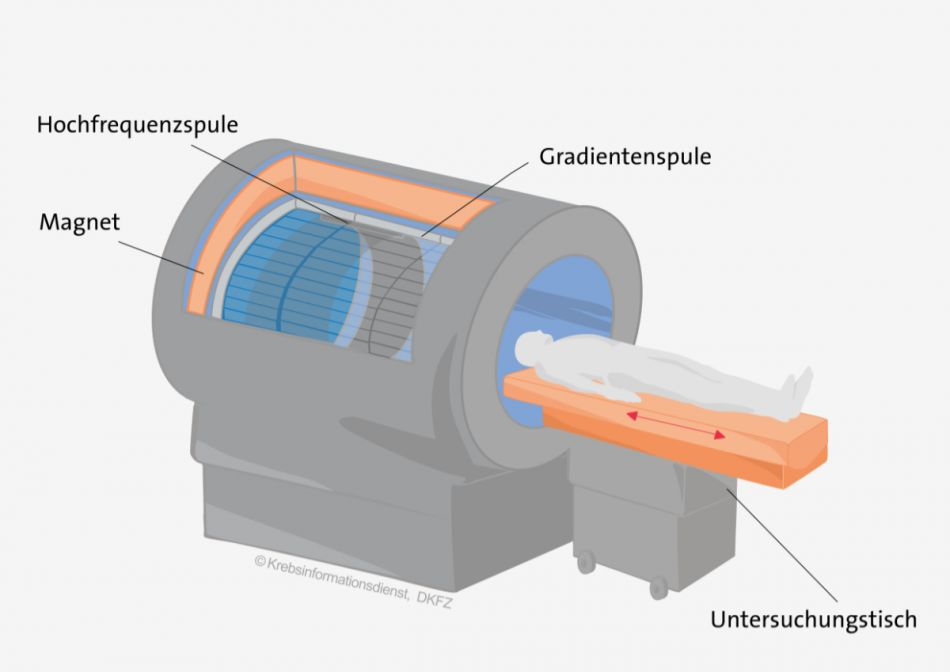
\includegraphics[width=.9\textwidth]{mrt_aufbau.jpg}
	\caption{Schematischer Aufbau eines Magnetresonanztomographen (Quelle: \url{https://www.krebsinformationsdienst.de/untersuchung/bildgebung/kernspintomographie.php})}
\end{figure}

Der Magnetresonanztomograph besteht aus mehreren Komponenten: 
\begin{itemize}
	\item einem supraleitenden Hauptmagneten in einer Röhre, der ein starkes und konstanten Magnetfeld erzeugt. Ein supraleitender Magnet wird durch flüssigen Stickstoff gekühlt, sodass der Spulenwiderstand nahezu null wird. Dies ermöglicht die Erzeugung starker Magnetfelder.
	\item einem Gradientensystem, das zusätzliche Magnetfelder generiert, die je nach Position im Körper unterschiedlich sind und so eine räumliche Auflösung ermöglichen.
	\item einem Hochfrequenzsystem, welches aus einem Sende- und Empfangsspulensystem besteht. Dieses sendet Radiowellen zur Anregung der Wasserstoffatome aus, welche dadurch ihrer Ausrichtung verlieren.
	\item einem Computersystem, das geeignet ist für die Verarbeitung der Daten eines \ac{MRT}s
	\item und einem Untersuchungstisch, auf welchem der Patient während der Untersuchung liegt
\end{itemize}
Das Verfahren basiert auf einem physikalischen Prinzip, dem Eigendrehimpuls auch Spin genannt. Dabei dreht sich ein \gls{Proton} um seinen eignen Schwerpunkt (Kernspin) und erzeugt durch die Rotation ein Magnetfeld. Die Wasserstoffkerne in unserem Körper besitzen ebenfalls einen Spin und verhalten sich so wie kleine Magnete, die ein messbares Magnetfeld erzeugen.\\
Die Kernspins sind im Normalzustand ungeordnet, legt man jedoch ein starkes Magnetfeld an, so richten sich die Kernspin-Achsen entlang den magnetischen Feldlinien aus. Sie führen dabei eine Kreiselbewegung aus, bei der sie sich immer näher an die Feldlinien bewegen, aber sich niemals ganz daran ausrichten, dies wird auch als Präzessionsbewegung bezeichnet. Die Frequenz dieser Bewegung nennt sich die Larmorfrequenz.\\ 
Allein durch die Ausrichtung der Kernspins erfolgt noch keine Bildgebung, es muss zunächst ein hochfrequenter Impuls (HF-Impuls) senkrecht zum Hauptmagnetfeld gegeben werden. Der Impuls muss dabei eine bestimmte Frequenz besitzen, nämlich die der Kernspins, also die Larmorfrequenz. Durch diesen Impuls synchronisieren sich die Protonen und manche der Kernspin-Achsen kippen um 90°, wobei sie bei diesem Vorgang Energie aufnehmen.\cite[vgl.][]{ChristophPabst2013}\\
Nach dem Impuls, kippen die Kernspins wieder zurück in ihre ursprüngliche Lage entlang des Hauptmagnetfeldes. Beim Ausrichten in die ursprüngliche Position, wird die aufgenommene Energie in Form von wärme wieder an die Umgebung abgegeben. Dieser Prozess der Wiederausrichtung wird als longitudinale Relaxation oder ``T1-Relaxation'' bezeichnet. Hierbei kommt es auf die Wärmeleitfähigkeit des Gewebes an. Ein weiterer Prozess der beim Ausschalten des HF-Impulses in Gang gesetzt wird, ist der Verlust der synchronen Kreiselbewegung, wodurch die transversal Magnetisierung verloren geht. Unterschiedliche Gewebe können die transversal Magnetisierung unterschiedlich lang aufrecht erhalten und erzeugen so Kontraste auf den Bildern, dies wird auch als ``T2-Relaxation'' bezeichnet. Man misst im wesentlichen die Dauer der verschiedenen Prozesse und kann anhand dessen auf die Gewebearten schließen und daraus die Kontraste berechnen.\cite[vgl.][]{Kernspin2022}

Es können zusätzlich Kontrastmittel verwendet werden, um bestimmte Teile heller erscheinen zulassen. Je nach Art des Kontrastmittels werden andere Bereicher dunkler, bzw. heller dargestellt. Die Kontrastmittel selbst sind nicht auf dem Bild zusehen, jedoch ihre Auswirkungen auf das umliegende Gewebe, so erscheint bei einer kontrastverstärkten T1-Gewichtung die Umgebung wie z.B. Blut oder Tumore heller. \cite[vgl.][]{ChristophPabst2013}

Es gibt weitere Methoden für eine \ac{MRT}, um bestimmte Strukturen, Gewebearten oder Flüssigkeiten heller bzw. dunkler erscheinen zu lassen. Eine davon ist die Flair-Gewichtung (fluid-attenuated inversion recovery), eine spezielle Methode zur Unterdrückung von Flüssigkeiten auf den entstehenden Bildern. Es unterdrückt z.B. das Liquor im Gehirn, wodurch bestimme Tumore besser sichtbar werden. Besitzt der Tumor jedoch einen hohen Wasseranteil, so wird dieser ebenfalls auf dem Bild unterdrückt. \cite[vgl.][]{Gizewski2001}